\chapter{Metodologia}
\label{chap:metodologia}
Este trabalho utiliza três frentes principais para alcançar os resultados propostos: (i) um mecanismo de aquisição e consolidação de requisitos do projeto elétrico residencial, capaz de interagir com o usuário em linguagem natural e/ou interpretar uma planta baixa em formato de imagem; (ii) um conjunto de rotinas de dimensionamento fundamentadas em normas técnicas aplicáveis a instalações elétricas de baixa tensão e em diretrizes locais de fornecimento, responsáveis por transformar as informações do imóvel em cálculos e decisões de projeto; e (iii) um procedimento de verificação de conformidade com realimentação do processo, visando assegurar que o resultado final atenda aos critérios normativos e às boas práticas adotadas.

Além disso, o método foi estruturado para manter rastreabilidade ao longo da execução, por meio de uma representação estruturada do projeto (modelo da residência), que é atualizada progressivamente conforme novas informações são obtidas e conforme os cálculos são realizados. Essa abordagem permite organizar o processo em etapas claras, reduzir ambiguidades e apoiar a geração final do memorial de cálculo.

Neste capítulo, serão detalhadas as metodologias empregadas para (a) coletar e organizar as entradas do usuário, (b) construir o modelo do imóvel, (c) executar o \textit{pipeline} de dimensionamento e (d) validar o atendimento às normas técnicas, culminando na geração do memorial de cálculo.

\section*{Solução proposta e visão geral do Fluxo}
\begin{landscape}
\begin{figure}[p]
	\centering
	\Caption{\label{fig:bpmn} Fluxo metodológico do agente para projeto elétrico residencial}	
	\UFCfig{}{
	    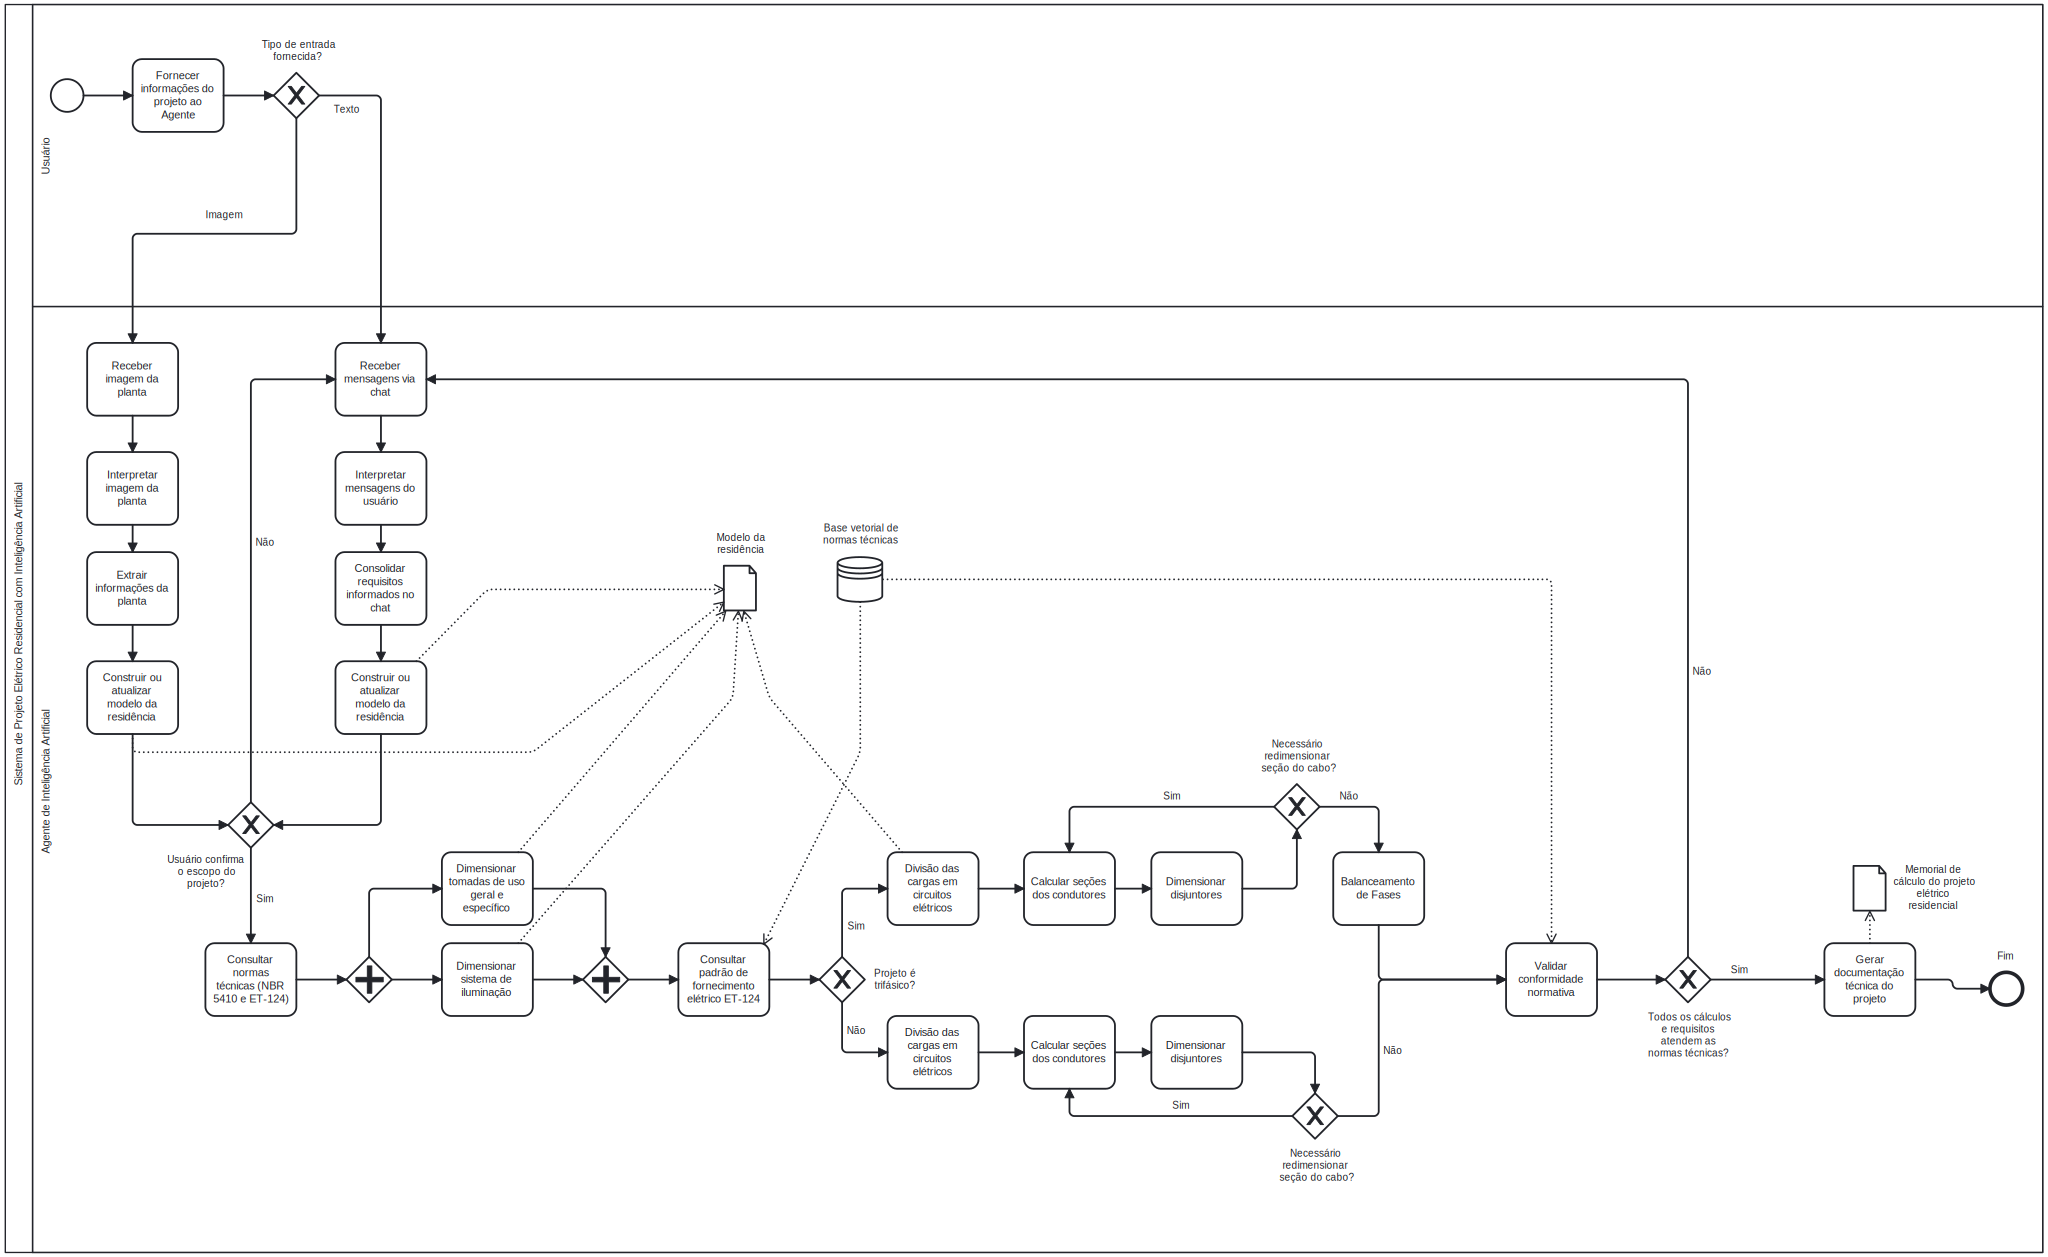
\includegraphics[width=\linewidth]{figuras/bpmn.png}
	}{
	    \Fonte{Elaborado pelo autor}
	}	
\end{figure}
\end{landscape}

A Figura \ref{fig:bpmn} apresenta o fluxo metodológico proposto neste trabalho, representado em formato processual. O processo, se inicia com o fornecimento de informações pelo usuário ao agente, podendo ocorrer por dois caminhos de entrada: texto (conversação em linguagem natural) ou imagem da planta baixa.



No primeiro caminho, o usuário interage por mensagens, e as informações são interpretadas e consolidadas progressivamente, até que o escopo do projeto seja suficientemente definido. No segundo caminho, o usuário fornece uma planta baixa em formato de imagem contendo, preferencialmente, identificação dos ambientes e suas dimensões. A interpretação da planta busca extrair os dados geométricos necessários ao dimensionamento; quando a extração não é satisfatória, o fluxo prevê mecanismos auxiliares de extração e normalização das informações. Em ambos os casos, as informações obtidas alimentam a construção e atualização do modelo da residência, que representa os ambientes e as cargas previstas, incluindo cargas específicas informadas pelo usuário ao longo da interação.

Uma vez consolidado o modelo do imóvel, o fluxo avança para as etapas de dimensionamento fundamentadas nas normas técnicas e diretrizes de fornecimento adotadas. Nessa fase, são executados, de forma sequencial e coerente, os cálculos relacionados a iluminação, tomadas de uso geral, tomadas de uso específico, bem como a divisão da instalação em circuitos terminais, com base em critérios normativos e boas práticas de projeto. A partir da definição dos circuitos, o processo realiza o dimensionamento de condutores e dispositivos de proteção, priorizando critérios de capacidade de condução de corrente e coerência entre condutor e proteção. Para instalações alimentadas por mais de uma fase, o fluxo prevê ainda o balanceamento de cargas entre fases, buscando o maior equilíbrio possível.

O diagrama também contempla pontos de decisão e realimentação. Caso seja identificado que algum critério não foi atendido (por exemplo, necessidade de ajuste de dimensionamento), o processo retorna às etapas apropriadas para correção. Ao final, é executada uma etapa de validação de conformidade normativa, na qual se verifica se os resultados atendem aos requisitos aplicáveis e às boas práticas adotadas. Somente após a validação positiva o fluxo segue para a geração do memorial de cálculo e demais tabelas finais do projeto, encerrando o processo.

\section{Aquisição das informações do projeto e consolidação do escopo}

O funcionamento do método proposto depende, inicialmente, da aquisição e estruturação das informações do projeto elétrico residencial. Nesta etapa, descrita na Figura \ref{fig:pt1}, o objetivo é transformar entradas não estruturadas (texto em linguagem natural e/ou imagem da planta) em um modelo de dados estruturado, contendo os parâmetros mínimos necessários para a execução dos dimensionamentos previstos no escopo do trabalho.

\begin{figure}[h!]
    \centering
    \Caption{\label{fig:pt1} Recorte do fluxo metodológico: aquisição de informações e consolidação do escopo}	
    \UFCfig{}{
	\includegraphics[width=0.5\textwidth]{figuras/pt1.png}
    }{
	\Fonte{Elaborado pelo autor}
    }	
\end{figure}

A aquisição das informações ocorre por dois caminhos: (i) interação conversacional e (ii) interpretação de planta baixa em formato de imagem. Em ambos os casos, o fluxo prevê mecanismos de confirmação e complementação, de modo que o escopo seja considerado “fechado” apenas quando o modelo do imóvel estiver completo o suficiente para dar início aos cálculos.

\subsection{Entrada por conversação em linguagem natural}
No modo conversacional, detalhado na Figura \ref{fig:pt1texto}, o usuário descreve características do imóvel e do fornecimento por meio de mensagens em linguagem natural. O sistema conduz uma sequência de perguntas e confirmações para reduzir ambiguidade e coletar informações essenciais. Essa abordagem é particularmente útil quando o usuário não possui a planta em imagem ou quando existem dados que não estão explicitamente presentes na planta.

\begin{figure}[h!]
    \centering
    \Caption{\label{fig:pt1texto} Detalhe do fluxo: entrada por conversação em linguagem natural}	
    \UFCfig{}{
	\includegraphics[width=0.5\textwidth]{figuras/pt1texto.png}
    }{
	\Fonte{Elaborado pelo autor}
    }	
\end{figure}

As informações mínimas buscadas nessa etapa incluem:

\begin{itemize}
	\item tensão de alimentação adotada no projeto;

	\item método de instalação considerado (assumindo-se um método padrão, quando não especificado, com possibilidade de alteração);

	\item parâmetros gerais de projeto, como hipóteses de agrupamento e organização de circuitos;

	\item cargas específicas (tomadas de uso específico), informadas pelo usuário, que impactam diretamente a divisão de circuitos e o dimensionamento.
\end{itemize}

À medida que o diálogo avança, as informações são registradas no modelo de dados do projeto. Quando o usuário menciona a existência de uma carga dedicada (por exemplo, um equipamento com alimentação específica em determinado ambiente), essa carga passa a compor explicitamente o modelo do imóvel e será tratada nas etapas posteriores.

\subsection{Entrada por imagem da planta baixa}
No modo de entrada por imagem, ilustrado na Figura \ref{fig:pt1imagem}, o usuário fornece uma planta baixa que contenha, preferencialmente, identificação dos ambientes e dimensões (comprimento e largura). A partir dessa entrada, o sistema realiza a interpretação da planta para extrair dados geométricos relevantes ao dimensionamento, como:

\begin{figure}[h!]
    \centering
    \Caption{\label{fig:pt1imagem} Detalhe do fluxo: entrada por imagem da planta baixa}	
    \UFCfig{}{
	\includegraphics[width=0.3\textwidth]{figuras/pt1imagem.png}
    }{
	\Fonte{Elaborado pelo autor}
    }	
\end{figure}

\begin{itemize}
	\item lista de ambientes;

	\item dimensões dos ambientes;

	\item grandezas derivadas, como área e perímetro.

\end{itemize}

Quando a interpretação direta da imagem não é suficiente para extrair informações com qualidade, o método prevê um mecanismo auxiliar de extração textual como alternativa (fallback), permitindo recuperar rótulos e valores dimensionais presentes na planta. Em seguida, os dados extraídos são validados e normalizados antes de serem incorporados ao modelo do projeto.

Nesta versão do trabalho, a entrada por planta é limitada ao formato de imagem, sendo a extensão para outros formatos (por exemplo, arquivos CAD) considerada como possibilidade de trabalhos futuros.

\subsection{Estruturação do modelo do imóvel e regras de consistência}
Independentemente do canal de entrada, as informações coletadas são organizadas em um modelo estruturado do imóvel, composto, no mínimo, por:

\begin{itemize}
    \item parâmetros de alimentação (como tensão);
    \item relação de ambientes (nome e dimensões);
    \item grandezas geométricas derivadas (área e perímetro);
    \item registro de cargas previstas por ambiente, incluindo cargas específicas informadas durante a interação.
\end{itemize}

Além de armazenar os dados, a metodologia aplica regras de consistência para evitar propagação de erros para as etapas de cálculo, tais como:

\begin{itemize}
    \item verificação de dimensões válidas (valores positivos e coerentes);
    \item padronização de unidades e formatos numéricos;
    \item confirmação de informações sensíveis ao dimensionamento quando há ambiguidade (por exemplo, tensão de alimentação e presença de cargas dedicadas).
\end{itemize}

\subsection{Critério de encerramento da etapa (escopo “fechado”)}
Considera-se que o escopo está ``fechado'' quando o modelo do imóvel contém informações suficientes para iniciar o \textit{pipeline} de dimensionamento, isto é:

\begin{enumerate}
    \item parâmetros de alimentação definidos;
    \item ambientes identificados com dimensões válidas;
    \item cargas específicas relevantes registradas (quando existirem);
    \item ausência de lacunas que comprometam a divisão em circuitos e o dimensionamento por critérios do escopo.
\end{enumerate}

A partir desse ponto, o fluxo avança para as etapas de cálculo e validação normativa, mantendo a possibilidade de retorno à etapa de aquisição caso sejam identificadas inconsistências durante as verificações posteriores.

\section{Modelo normativo e estratégia de aplicação}
Com o escopo consolidado e o modelo do imóvel estruturado, o método avança para a etapa em que as informações coletadas são transformadas em decisões e cálculos do projeto elétrico residencial. Nesta fase, a metodologia adota como referência as normas técnicas aplicáveis a instalações elétricas de baixa tensão e as diretrizes locais de fornecimento, estabelecendo um conjunto de regras e critérios que guiam o dimensionamento, com base na ABNT NBR 5410 \cite{NBR5410:2004, NBR5410:2008}.

A estratégia adotada combina dois elementos complementares:
(i) rotinas determinísticas de dimensionamento, que formalizam regras normativas em procedimentos reprodutíveis; e
(ii) um mecanismo de consulta e fundamentação normativa \cite{Lewis2020}, utilizado para justificar escolhas e responder dúvidas do usuário sobre o porquê de determinadas decisões.

Essa abordagem é relevante porque o dimensionamento elétrico possui partes estritamente normativas e calculáveis, que demandam consistência e repetibilidade, e também possui pontos em que o usuário necessita de esclarecimento técnico sobre critérios adotados e boas práticas.

\subsection{Formalização das regras normativas}
As regras extraídas dos documentos técnicos são organizadas em rotinas de cálculo e critérios de verificação. Sempre que uma regra puder ser expressa de forma objetiva (por exemplo, cálculo de cargas mínimas, definição de limites por circuito, obrigatoriedade de circuitos exclusivos para determinadas cargas), ela é incorporada como procedimento determinístico. Dessa forma, o método garante que, para um mesmo conjunto de entradas, os resultados produzidos serão consistentes e auditáveis.

Quando houver necessidade de esclarecer decisões (por exemplo, justificar a separação de circuitos, explicar limites de potência adotados ou a razão de circuitos dedicados), o método utiliza a consulta a trechos normativos e diretrizes aplicáveis como suporte explicativo. Assim, a fundamentação técnica pode ser apresentada de forma transparente, sem comprometer a consistência do dimensionamento.

\subsection{Organização do \textit{pipeline} de dimensionamento}

O dimensionamento é estruturado em etapas sequenciais, refletindo o fluxo de projeto e reduzindo dependências circulares, conforme detalhado na Figura \ref{fig:pipeline}. De forma geral, o \textit{pipeline} é organizado como:

\begin{enumerate}
    \item \textit{Cálculo das cargas por ambiente:} determinação das cargas mínimas de iluminação e das cargas de tomadas de uso geral (TUG) por ambiente, conforme regras normativas para cada tipo de cômodo.
    \item \textit{Incorporação de cargas específicas (TUE):} registro de cargas informadas pelo usuário que devem receber tratamento dedicado no projeto.
    \item \textit{Divisão em circuitos terminais:} organização da instalação em circuitos de iluminação e circuitos de tomadas, com separação funcional e aplicação de critérios normativos e boas práticas para limitação de potência por circuito, quando necessário.
    \item \textit{Dimensionamento de condutores:} seleção da seção dos condutores por circuito, considerando como critério principal a capacidade de condução de corrente, dadas as premissas adotadas (material do condutor, tipo de isolação, método de instalação e condições de referência).
    \item \textit{Dimensionamento dos dispositivos de proteção:} escolha dos dispositivos de proteção compatíveis com os circuitos dimensionados, preservando coerência técnica entre proteção e condutores.
    \item \textit{Balanceamento de fases (quando aplicável):} distribuição dos circuitos entre fases buscando equilíbrio de potência por fase, conforme boas práticas e diretrizes aplicáveis.
    \item \textit{Verificação de conformidade e ajustes:} checagem do atendimento às regras adotadas, com retorno às etapas anteriores quando necessário.
\end{enumerate}

Cada uma dessas etapas produz saídas intermediárias que são armazenadas de forma estruturada, permitindo rastreabilidade e facilitando a geração do memorial de cálculo ao final do processo.

\subsection{Premissas e limites de escopo adotados}
Para tornar o método objetivo e reprodutível, foram adotadas premissas compatíveis com o contexto residencial, incluindo um método de instalação de referência e condições padrão para o dimensionamento por capacidade de condução de corrente. Nesta versão do trabalho, o dimensionamento é centrado em critérios diretamente aplicáveis às etapas de cálculo, divisão de circuitos, seleção de condutores e proteção, além do balanceamento quando pertinente.

Critérios adicionais, como verificação de queda de tensão, curto-circuito e aterramento, não são contemplados no escopo atual e são indicados como extensões futuras, sem prejuízo ao objetivo principal do trabalho.

\section{\textit{Pipeline} de dimensionamento do projeto elétrico}
\label{sec:pipeline}
O dimensionamento do projeto elétrico residencial proposto neste trabalho é conduzido por um \textit{pipeline} sequencial, ilustrado na Figura \ref{fig:pipeline}, fundamentado na previsão de cargas mínimas e na organização em circuitos terminais, conforme critérios normativos e boas práticas usuais. O levantamento das potências é realizado por meio de uma previsão das cargas mínimas de iluminação e tomadas, permitindo determinar a potência total prevista da instalação. Essa previsão segue o que estabelece o item 9.5.2 da ABNT NBR 5410 \cite{NBR5410:2004}, que orienta o procedimento de estimativa das cargas a serem instaladas.

\begin{figure}[h!]
    \centering
    \Caption{\label{fig:pipeline} \textit{Pipeline} de dimensionamento do projeto elétrico}	
    \UFCfig{}{
	\includegraphics[width=\textwidth]{figuras/pipeline.png}
    }{
	\Fonte{Elaborado pelo autor}
    }	
\end{figure}

\subsection{Previsão de carga de iluminação}
A carga mínima de iluminação por cômodo/dependência é estimada em função da área do ambiente, conforme o \textit{item 9.5.2} da ABNT NBR 5410 \cite{NBR5410:2004}. Para fins de aplicação metodológica, adota-se:

\begin{itemize}
    \item Para ambientes com área $\le$ 6 m$^2$: prever 100 VA de carga mínima de iluminação.
    \item Para ambientes com área $>$ 6 m$^2$: prever 100 VA para os primeiros 6 m$^2$ acrescida de 60 VA a cada aumento de 4 m$^2$ inteiros.
\end{itemize}

Essa regra permite que a carga mínima de iluminação seja calculada de forma reprodutível a partir das dimensões do cômodo, gerando como saída: (i) potência de iluminação por ambiente e (ii) potência total de iluminação da residência.

\textit{Observação normativa:} além da potência, a norma estabelece que, para cada cômodo ou dependência, deve ser previsto pelo menos um ponto de luz fixo no teto, comandado por interruptor, conforme o \textit{subitem 9.5.2.1.1} da ABNT NBR 5410 \cite{NBR5410:2004}.

\subsection{Previsão de tomadas de uso geral}
A previsão de TUG é realizada conforme o item 9.5.2 da ABNT NBR 5410 \cite{NBR5410:2004}, diferenciando-se por tipo de ambiente. Além disso, no caso de banheiros e demais situações com restrições, deve-se respeitar as condições de instalação indicadas no item 9.1 (restrições/zonas aplicáveis ao ambiente).

De forma resumida, a metodologia aplica:

\begin{itemize}
    \item \textit{Banheiros:} prever pelo menos 1 tomada próxima ao lavatório, respeitando as restrições do item 9.1; atribuir 600 VA por tomada (mínimo).
    \item \textit{Cozinhas, copas, copas-cozinhas, áreas de serviço, lavanderias e locais semelhantes:} prever no mínimo 1 tomada a cada 3,5 m de perímetro (ou fração); atribuir 600 VA por ponto para até 3 pontos e 100 VA por ponto excedente, considerando cada ambiente separadamente.
    \item \textit{Varandas:} prever pelo menos 1 tomada (admitindo-se posição próxima ao acesso em situações construtivas específicas); atribuir 100 VA por tomada.
    \item \textit{Salas e dormitórios:} prever no mínimo 1 tomada a cada 5 m de perímetro (ou fração); atribuir 100 VA por tomada.
    \item \textit{Demais cômodos/dependências:} se área $\le$ 6 m$^2$, prever ao menos 1 tomada; se área $>$ 6 m$^2$, prever 1 tomada a cada 5 m de perímetro (ou fração); atribuir 100 VA por tomada.
\end{itemize}

Como saída dessa etapa, o método obtém a quantidade mínima de TUG por ambiente, a potência atribuída por ambiente e o total de TUG da instalação.

\begin{table}[h!]	
	\centering
	\Caption{\label{tab:regras_tug} Regras mínimas de previsão de TUG por tipo de ambiente e potência atribuída}
	\UFCtab{}{
		\resizebox{\linewidth}{!}{
			\begin{tabular}{lp{7cm}l}
			\toprule
	    		Tipo de ambiente & Regra mínima de quantidade & Potência atribuída \\
			\midrule \midrule
				Banheiros & Pelo menos 1 tomada próxima ao lavatório (ver item 9.1) & $\ge$ 600 VA por tomada \\
				\addlinespace
				Cozinhas, copas, áreas de serviço e semelhantes & 1 tomada a cada 3,5 m de perímetro (ou fração), independente da área & 600 VA até 3 pontos; 100 VA p/ excedente \\
				\addlinespace
				Varandas & Pelo menos 1 tomada (admite-se próxima ao acesso) & 100 VA por tomada \\
				\addlinespace
				Salas e dormitórios & 1 tomada a cada 5 m de perímetro (ou fração), independente da área & 100 VA por tomada \\
				\addlinespace
				Demais cômodos & Área $\le$ 6 m$^2$: 1 tomada; Área $>$ 6 m$^2$: 1 a cada 5 m de perímetro & 100 VA por tomada \\
			\bottomrule
		\end{tabular}
		}
	}{
		\Fonte{Adaptado de ABNT \cite{NBR5410:2004}.}
    }
\end{table}

Com base nas regras de previsão de carga mínima de iluminação (item 9.5.2) e nas regras de TUG sintetizadas na Tabela \ref{tab:regras_tug} obtém-se a carga prevista de TUG por ambiente e a carga total de TUG da instalação, as quais são utilizadas nas etapas posteriores de divisão em circuitos terminais e dimensionamento.

\subsection{Tomadas de uso específico - TUE e circuitos dedicados}
As cargas específicas (TUE) são incorporadas ao modelo do projeto a partir das informações fornecidas pelo usuário (ex.: condicionador de ar, chuveiro elétrico, máquina de lavar). Conforme o \textit{subitem 9.5.3.1} da ABNT NBR 5410 \cite{NBR5410:2004}, todo ponto de utilização previsto para alimentar equipamento de modo exclusivo ou virtualmente dedicado, com corrente nominal superior a 10 A, deve constituir um circuito independente.

Na prática metodológica, isso implica:

\begin{itemize}
    \item registrar cada TUE com sua localização (ambiente) e característica de potência/corrente;
    \item alocar cada TUE em circuito terminal próprio, evitando compartilhamento com TUG;
    \item permitir (por critério de projetista) a criação de circuitos dedicados também para cargas com corrente inferior a 10 A quando houver justificativa técnica (por exemplo, natureza motriz ou sensibilidade eletrônica), mantendo coerência com a boa prática.
\end{itemize}
\subsection{Divisão da instalação em circuitos terminais}

Com as cargas mínimas de iluminação e TUG calculadas e as TUE consolidadas, realiza-se a divisão da instalação em circuitos terminais. Essa divisão visa facilitar operação e manutenção, permitir seccionamento adequado e reduzir interferência entre pontos de utilização.

A metodologia aplica:

\begin{enumerate}
    \item[\textbf{(a)}] \textit{Separação funcional:} circuitos de iluminação devem ser separados de circuitos de tomadas de uso geral (boa prática consistente com projetos residenciais) \cite{Creder2016}.
    
    \item[\textbf{(b)}] \textit{Circuitos exclusivos para TUE (subitem 9.5.3.1):} TUE alocadas em circuitos independentes quando aplicável (corrente nominal $> 10$ A ou carga dedicada/virtualmente dedicada).
    
    \item[\textbf{(c)}] \textit{Tomadas de cozinhas e áreas semelhantes (item 9.5.3.2):} os pontos de tomada de cozinhas, copas-cozinhas, áreas de serviço, lavanderias e locais semelhantes devem ser atendidos por circuitos destinados exclusivamente às tomadas desses locais.
    
    \item[\textbf{(d)}] \textit{Limitação de potência por circuito:} para manter o projeto coerente com faixas usuais de proteção, adota-se a limitação de potência como boa prática \cite{Mamede2017}:
    \begin{itemize}
        \item \textit{Iluminação:} limitar a potência por circuito conforme prática didática e valores de referência por tensão.
        \item \textit{TUG:} limitar a potência por circuito considerando a capacidade dos dispositivos de proteção e condutores.
    \end{itemize}
    \textit{Nota: Quando a potência total se mantém abaixo dos limites de referência, admite-se manter um único circuito, respeitadas as separações funcionais.}

    \item[\textbf{(e)}] \textit{Distribuição entre fases:} em instalações bifásicas ou trifásicas, as cargas devem ser distribuídas buscando o maior equilíbrio possível entre as fases.
\end{enumerate}

\subsubsection{Regra para determinação do número de circuitos}
\label{subsubsec:met_regra_circuitos}

Para traduzir as diretrizes normativas em um procedimento computável pelo agente, adotou-se a seguinte lógica sequencial para a definição da quantidade e disposição dos circuitos terminais:

\textbf{1. Circuitos de segregação obrigatória:}
Antes do agrupamento por potência, as cargas são classificadas em grupos funcionais rígidos ($g$), conforme a NBR 5410:
\begin{itemize}
    \item \textbf{Iluminação:} Separada totalmente de tomadas;
    \item \textbf{TUG (Cozinhas e Áreas de Serviço):} Devem formar circuitos exclusivos, não misturados com salas ou quartos;
    \item \textbf{TUE:} Cada TUE identificada gera automaticamente um circuito independente ($n_{TUE} = 1$).
\end{itemize}

\textbf{2. Quantidade por limite de potência:}
Para os grupos de iluminação e TUGs, o número mínimo de circuitos ($n_g$) é determinado dividindo-se a potência total do grupo ($S_{g,\text{total}}$) por uma potência limite de referência ($S_{g,\text{lim}}$). Adotaram-se como valores de referência para tensão de 220 V: $S_{lim,ilum} \approx 2500$ VA e $S_{lim,TUG} \approx 4300$ VA (baseado em disjuntores de até 20 A). A quantidade é dada por:

\begin{equation}
    n_g = \max\left(1, \left\lceil \frac{S_{g,\text{total}}}{S_{g,\text{lim}}} \right\rceil\right)
\end{equation}

Onde $\lceil x \rceil$ representa a função teto (menor inteiro maior ou igual a $x$).

\textbf{3. Algoritmo de particionamento:}
O agente distribui as cargas entre os $n_g$ circuitos utilizando uma abordagem gulosa (\textit{greedy}): ordena-se as cargas por ambiente para manter a contiguidade espacial e aloca-se carga a um circuito até que a adição da próxima exceda $S_{g,\text{lim}}$. Nesse caso, encerra-se o circuito atual e abre-se um novo.

\textbf{4. Verificação de corrente:}
Após a divisão, calcula-se a corrente de projeto ($I_B$) de cada circuito. Caso algum circuito exceda a capacidade típica de disjuntores terminais de uso geral (ex.: 20 A para TUG), o algoritmo incrementa $n_g$ e redistribui as cargas.

\textbf{Exemplo de aplicação:}
Considerando um agrupamento de TUGs de dormitórios e salas com $S_{g,\text{total}} = 7200$ VA (em 220 V) e adotando o limite de referência $S_{lim} = 4300$ VA. O sistema calcula $n = \lceil 7200/4300 \rceil = \lceil 1,67 \rceil = 2$ circuitos. As tomadas são então distribuídas entre estes dois circuitos, priorizando que tomadas do mesmo cômodo permaneçam no mesmo circuito sempre que possível.
\subsection{Previsão de circuitos reserva}
O método prevê reserva para ampliações futuras sob dois aspectos complementares:
\begin{itemize}
	\item reserva física no quadro de distribuição (espaço para inclusão de disjuntores/circuitos);


	\item reserva de potência associada a circuitos típicos (valores usuais adotados por critério de projetista em práticas acadêmicas e profissionais).

\end{itemize}

\subsection{Dimensionamento de condutores e dispositivos de proteção}
Após a definição dos circuitos terminais, estima-se a corrente por circuito a partir da potência atribuída e da tensão do projeto. Em seguida:
\begin{itemize}
	\item dimensionam-se os condutores pelo critério principal de capacidade de condução de corrente (ampacidade), adotando premissas usuais do escopo (material e isolação usuais, método de instalação de referência e condições padrão);

	\item selecionam-se os dispositivos de proteção coerentes com o circuito dimensionado, assegurando compatibilidade entre proteção e condutor.
\end{itemize}
\subsection{Balanceamento de fases}
Quando aplicável, o balanceamento é realizado visando equilibrar a potência por fase, distribuindo circuitos de modo a reduzir assimetrias. Circuitos dedicados (TUE) são tratados como elementos prioritários, a fim de evitar repartições inadequadas e preservar a lógica funcional do projeto.
\subsection{Verificação final e retorno para correções}
Ao final do \textit{pipeline}, verifica-se o atendimento às regras normativas citadas (itens 9.5.2, 9.5.2.1.1, 9.1, 9.5.3.1 e 9.5.3.2) e às boas práticas adotadas. Caso alguma inconsistência seja detectada (por exemplo, circuito excedendo limite de potência de referência ou TUE não dedicada), o fluxo retorna à etapa pertinente (divisão de circuitos ou dimensionamento), até que o conjunto final esteja coerente para geração do memorial.


\section{Geração do memorial de cálculo e organização da documentação do projeto}
Concluídas as etapas de previsão de cargas, divisão em circuitos terminais e dimensionamento, os resultados são consolidados em um memorial de cálculo. Esse documento tem por finalidade registrar, de forma organizada e rastreável, as premissas adotadas, os critérios normativos utilizados e os principais resultados obtidos, permitindo verificação técnica e comunicação clara do projeto.

O memorial gerado segue uma estrutura padronizada, organizada em seções que refletem diretamente o \textit{pipeline} descrito na Seção \ref{sec:pipeline}, garantindo coerência entre: (i) informações de entrada, (ii) resultados intermediários e (iii) dimensionamento final.

\subsection{Organização do memorial}
O memorial é composto, de modo geral, pelas seguintes seções:

\begin{enumerate}
    \item \textit{Dados da obra} \\
    Identificação da edificação, localização, tipo de uso e dados básicos do projeto. Essa seção também inclui campos para identificação do(s) projetista(s) e informações de fornecimento quando aplicável.

    \item \textit{Objetivos e escopo do memorial} \\
    Apresenta o objetivo do documento e delimita o escopo do projeto gerado, tipicamente incluindo:
    \begin{itemize}
        \item definição e quantificação de cargas por ambiente;
        \item cálculo da potência instalada prevista;
        \item divisão em circuitos terminais;
        \item dimensionamento de condutores e especificação das proteções;
        \item diretrizes de organização do quadro e registros necessários para execução.
    \end{itemize}

    \item \textit{Metodologia aplicada no memorial} \\
    Resume os critérios adotados para levantamento de cargas e dimensionamento, com referência direta aos itens normativos que fundamentam as regras aplicadas. Em especial:
    \begin{itemize}
        \item previsão de cargas mínimas de iluminação e tomadas conforme ABNT NBR 5410 (item 9.5.2);
        \item obrigatoriedade de ponto de luz fixo por ambiente conforme subitem 9.5.2.1.1;
        \item regras de TUG por tipo de ambiente, com observação de restrições de instalação em ambientes específicos conforme item 9.1 quando aplicável;
        \item critério de circuitos dedicados para TUE conforme subitem 9.5.3.1;
        \item necessidade de circuitos exclusivos para tomadas de cozinhas/áreas similares conforme item 9.5.3.2;
        \item critérios de dimensionamento de condutores por capacidade de condução de corrente e seções mínimas, conforme os itens aplicáveis da ABNT NBR 5410.
    \end{itemize}

    \item \textit{Levantamento de cargas (por ambiente)} \\
    Apresenta tabelas por dependência com: área, perímetro, quantidade de pontos e potência mínima prevista para:
    \begin{itemize}
        \item iluminação (com base no item 9.5.2);
        \item TUG (com base no item 9.5.2 e restrições do item 9.1 quando aplicável);
        \item TUE (quando houver), registrando a carga nominal informada para cada equipamento.
    \end{itemize}
    Ao final, o memorial consolida um quadro-resumo de cargas e a potência total prevista.

    \item \textit{Divisão dos circuitos terminais} \\
    Documenta a etapa de agrupamento das cargas em circuitos, explicitando:
    \begin{itemize}
        \item separação entre iluminação e tomadas;
        \item criação de circuitos exclusivos para TUE (subitem 9.5.3.1);
        \item circuitos exclusivos para cozinhas/áreas similares (item 9.5.3.2);
        \item aplicação de limites de potência por circuito como boa prática;
        \item registro de circuitos reserva.
    \end{itemize}

    \item \textit{Padrão de fornecimento e dimensionamento da entrada/proteção geral} \\
    Com base na potência instalada prevista e nos critérios aplicáveis da concessionária local, registra: tipo de fornecimento (monofásico/bifásico/trifásico), proteção geral e seção mínima do condutor de entrada.

    \item \textit{Balanceamento de cargas (quando aplicável)} \\
    Apresenta a distribuição dos circuitos e um resumo das potências por fase, buscando o equilíbrio de potência.

    \item \textit{Dimensionamento dos condutores} \\
    Apresenta o dimensionamento por circuito contendo: potência, tensão, corrente de projeto e seção final selecionada, incluindo condutores neutro e de proteção.

    \item \textit{Dimensionamento dos dispositivos de proteção} \\
    Documenta a seleção do dispositivo de proteção por circuito, registrando o critério de coordenação entre corrente de projeto, corrente nominal do dispositivo e capacidade do condutor através das inequações normativas.

    \item \textit{Resumo consolidado} \\
    Consolida em tabelas finais: resumo por dependência, resumo por circuito, tabela completa de dimensionamento e resumo do fornecimento geral.
\end{enumerate}

\subsection{Rastreabilidade entre método e documento}
A estrutura do memorial é construída para manter correspondência direta com o \textit{pipeline} descrito na Seção \ref{sec:pipeline} e ilustrado na Figura \ref{fig:pipeline}. Assim, cada tabela do memorial deriva de uma etapa do método (cargas → circuitos → condutores → proteções → fornecimento/balanceamento), permitindo auditoria e verificação dos resultados obtidos.

\section{Estratégia de validação da metodologia}
A validação da metodologia proposta foi conduzida por meio de um estudo de caso, no qual os resultados gerados pelo método foram comparados com referências acadêmicas consolidadas no contexto de instalações elétricas residenciais. O objetivo dessa validação é verificar se as saídas produzidas, tais como previsão de cargas mínimas, divisão em circuitos terminais, dimensionamento de condutores, seleção de dispositivos de proteção e, quando aplicável, balanceamento de fases, permanecem coerentes com os critérios normativos e com práticas de projeto utilizadas no ensino de engenharia elétrica.

\subsection{Base de referência e dados utilizados}
Como referência principal, foi adotado um projeto elétrico residencial disponibilizado em contexto didático no curso de instalações elétricas residenciais da Universidade Federal do Ceará (UFC) \cite{ApostilaUFC, UFC_Prediais_ManualPraticas_2025}, que inclui enunciado do projeto, solução de referência (gabarito do docente) e soluções típicas produzidas por discentes. Essa escolha se justifica por se tratar de material estruturado com finalidade pedagógica e alinhado às exigências normativas, permitindo uma comparação objetiva entre o resultado esperado e o resultado obtido pela metodologia.

A entrada do estudo de caso foi composta pelas informações essenciais do imóvel (ambientes e dimensões) e pelos parâmetros de fornecimento e premissas usuais de projeto (por exemplo, tensão e condições de instalação de referência), de modo a reproduzir condições equivalentes às utilizadas no exercício acadêmico.

\subsection{Critérios de avaliação e equivalência aceitável}
A comparação entre os resultados foi feita considerando dois níveis:
\begin{alineascomnumero}
	    \item Conformidade normativa: verificação do atendimento aos requisitos e critérios prescritos na ABNT NBR 5410 aplicáveis às etapas contempladas no escopo do trabalho, incluindo a previsão de cargas mínimas, regras de pontos de tomada e pontos de iluminação, e requisitos de circuitos dedicados e separação funcional.
	    \item Equivalência de projeto (critério de projetista): reconhecimento de que, mesmo com atendimento normativo, podem existir variações legítimas de projeto. Assim, foram considerados equivalentes resultados que, embora não idênticos em todos os detalhes ao gabarito, permanecem tecnicamente aceitáveis.
\end{alineascomnumero}

Esse critério é relevante especialmente na divisão de circuitos, onde diferentes agrupamentos podem ser adotados sem violar requisitos, desde que sejam respeitadas as regras de separação, exclusividade quando exigida e limites de potência/corrente aplicáveis.
